\documentclass[12]{article}
% --------------------------------------------------------------
% This is all preamble stuff that you don't have to worry about.
% Head down to where it says "Start here"
% --------------------------------------------------------------
 
%\documentclass[12pt]{article}

\usepackage[margin=1in]{geometry} 
\usepackage{amsmath,amsthm,amssymb}
\usepackage[margin=1in]{geometry} 
\usepackage{amsmath,amsthm,amssymb}
\usepackage[English]{babel} %Castellanización
\usepackage[T1]{fontenc} %escribe lo del teclado
\usepackage[utf8]{inputenc} %Reconoce algunos símbolos
\usepackage{lmodern} %optimiza algunas fuentes
\usepackage{graphicx}
\graphicspath{ {images/} }
\usepackage{hyperref} % Uso de links
%\usepackage{apacite} 
\usepackage{mathtools}
\DeclarePairedDelimiter\bra{\langle}{\rvert}
\DeclarePairedDelimiter\ket{\lvert}{\rangle}
\DeclarePairedDelimiterX\braket[2]{\langle}{\rangle}{#1 \delimsize\vert #2}
\usepackage{mathrsfs}
\usepackage{amsmath}
\usepackage{xcolor}
\usepackage{lmodern} %optimiza algunas fuentes
\usepackage{titling} % Enables \subtitle command
\usepackage{subfig}
\usepackage{hyperref}


\newcommand{\N}{\mathbb{N}}
\newcommand{\Z}{\mathbb{Z}}
 
\newenvironment{theorem}[2][Theorem]{\begin{trivlist}
\item[\hskip \labelsep {\bfseries #1}\hskip \labelsep {\bfseries #2.}]}{\end{trivlist}}
\newenvironment{lemma}[2][Lemma]{\begin{trivlist}
\item[\hskip \labelsep {\bfseries #1}\hskip \labelsep {\bfseries #2.}]}{\end{trivlist}}
\newenvironment{exercise}[2][Exercise]{\begin{trivlist}
\item[\hskip \labelsep {\bfseries #1}\hskip \labelsep {\bfseries #2.}]}{\end{trivlist}}
\newenvironment{problem}[2][Problem]{\begin{trivlist}
\item[\hskip \labelsep {\bfseries #1}\hskip \labelsep {\bfseries #2.}]}{\end{trivlist}}
\newenvironment{question}[2][Question]{\begin{trivlist}
\item[\hskip \labelsep {\bfseries #1}\hskip \labelsep {\bfseries #2.}]}{\end{trivlist}}
\newenvironment{corollary}[2][Corollary]{\begin{trivlist}
\item[\hskip \labelsep {\bfseries #1}\hskip \labelsep {\bfseries #2.}]}{\end{trivlist}}

\newenvironment{solution}{\begin{proof}[Solution]}{\end{proof}}

 
\begin{document}
 
% --------------------------------------------------------------
%                         Start here
% --------------------------------------------------------------
%\color{blue}

\title{Metallic Materials - Metal Diffusion}
\author{Cap Morales, Shannon Nazareth\\
N25MA13}

\maketitle



\section{}

\subsection{}
\textbf{A Pb–$60$ at\% Sn alloy was slowly cooled from $380^{\circ}$C to $50^{\circ}$C. Calculate the volume fraction of the primary phase at $50^{\circ}$C.}

The phase diagram for an alloy of Pb and Sn is shown in figure \ref{fig:diagrama}. The temperature and composition are located in the diagram, the composition $C_0$ corresponds to a $60$\% of Sn and $40$\% of Pb. From the figure, it can be seen that for a temperature of $50^{\circ}$C there is presence of two phases, $\alpha$ and $\beta$. From the isothermal of the temperature it is possible to obtain the values of the compositions for each phase by intersecting the ishothermal llinea with the baoundaries of the phase diagram, which gives the following results:

\begin{align}
    \label{eq:compostitions}
    \begin{split}
        C_{Sn_{\alpha}}&=4\% \\ C_{Sn_{\beta}}&=99\% \\ C_{Pb_{\alpha}}&=96\% \\ C_{Pb_{\beta}}&=1\%,
    \end{split}
\end{align}
where $C_{Sn_{\alpha}}$ is the composition of Sn in the $\alpha$ phase, $C_{Sn_{\beta}}$ is the composition of Sn in the $\beta$ phase, $C_{Pb_{\alpha}}$ the composition of Pb in the $\alpha$ phase and, $C_{Pb_{\beta}}$ is the composition of Pb in the $\beta$ phase.

The primary phase is the phase that has a higher fraction in the mixture, for which is necessary to calcualte the fraction of each phase, and to do that the lever rule is used. The lever rule states that the phase fraction can be calculated taking the distance of the tie line of the total composition to the border of the other phase and divide this by the total distance of the tie line, the expressions for the mass fractions are presented in the following equations:

\begin{align}
    \label{eq:frac_alpha}
    W_{\alpha}&=\dfrac{C_{\beta}-C_0}{C_{\beta}-C_{\alpha}}
\end{align}
and
\begin{align}
    \label{eq:frac_beta}
    W_{\beta}&=\dfrac{C_0-C_{\alpha}}{C_{\beta}-C_{\alpha}};
\end{align}
where $W_{\alpha}$ is the fraction of the $\alpha$ phase, $W_{\beta}$ is the fraction of the $\beta$ phase, $C_{\alpha}$ and $C_{\beta}$ are the compositions of the $\alpha$ and $\beta$ phases, and $C_0$ is the initial composition \citep[p.~290-291]{callister2010materials}. 

\begin{figure}[h]
    \centering
    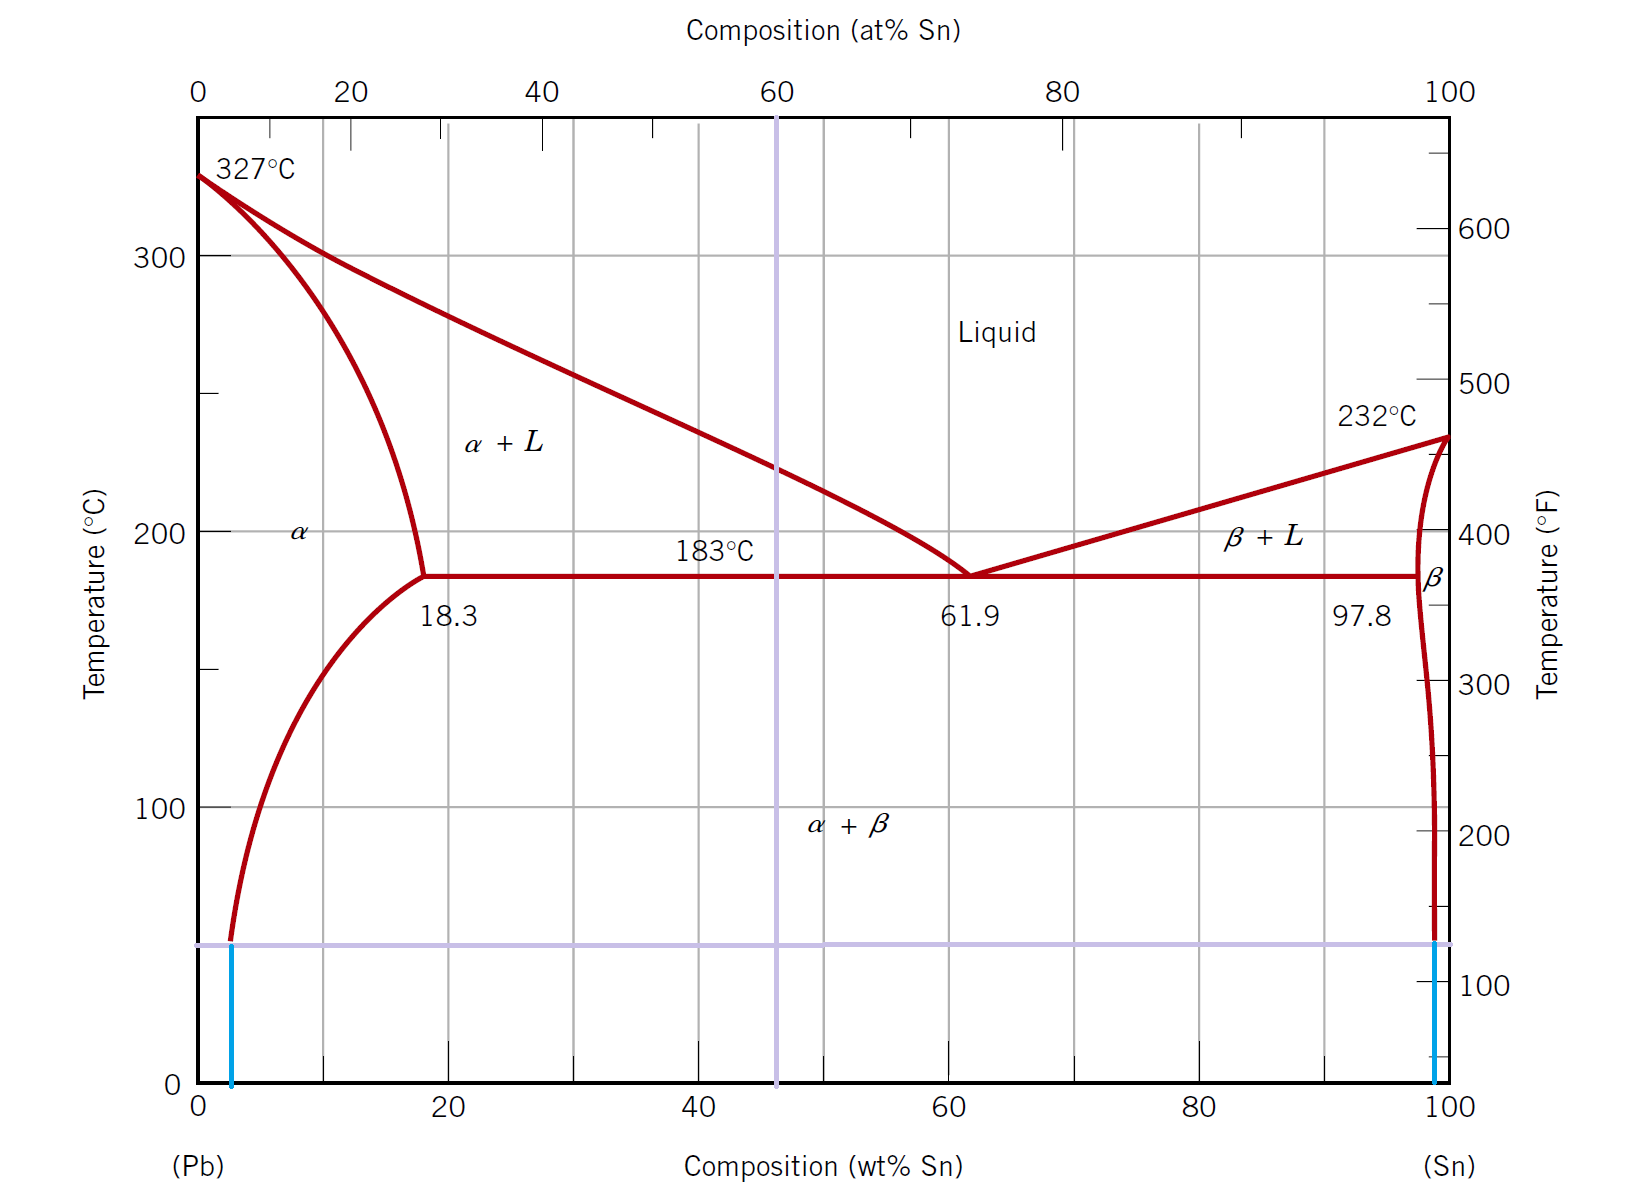
\includegraphics[width=0.93\textwidth]{graficas/diagrama.png}
    \caption{Phase diagram for lead-tin \\
    \textit{Source: Figure adapted from \citep{callister2010materials}}}
    \label{fig:diagrama}
\end{figure}

Using the values of the compositions for Sn from equation \ref{eq:compostitions} obtained from the phase diagram in figure \ref{fig:diagrama}, the fractions for $\alpha$ and $\beta$ phases are calculated using equations \eqref{eq:frac_alpha} and \eqref{eq:frac_beta}:

\begin{align}
    \label{eq:w_alpha}
    W_{\alpha}&=\dfrac{C_{\beta}-C_0}{C_{\beta}-C_{\alpha}} =\dfrac{99-60}{99-4} = \dfrac{39}{95} = 0.410526
\end{align}

\begin{align}
    \label{eq:w_beta}
    W_{\beta}&=\dfrac{C_0-C_{\alpha}}{C_{\beta}-C_{\alpha}} =\dfrac{60-4}{99-4} =\dfrac{59}{95} =0.589474
\end{align}

Based on the results obtained, it can be determined that the primary phase, the one that has a higher fraction, is the $\beta$ phase. The equation for the volumen fraction for the $\beta$ phase is given by:

\begin{align}
    \label{eq:vol_beta}
    V_{\beta}&=\dfrac{\dfrac{W_{\beta}}{\rho_{\beta}}}{\dfrac{W_{\alpha}}{\rho_{\alpha}}+\dfrac{W_{\beta}}{\rho_{\beta}}},
\end{align}
where $V_{\beta}$ is the volumen fraction of the $\beta$ phase, $W_{\alpha}$ and $W_{\beta}$ are the fractions of both $\alpha$ and $\beta$ phases, and $\rho_{alpha}$ and $\rho_{\beta}$ are the densities of $\alpha$ and $\beta$ phases respectively \citep[p.~293]{callister2010materials}.

From equation \eqref{eq:vol_beta} it can be seen that it is necessary to calculate the density of each phase, which can be done by using the following equations:

\begin{align}
    \label{eq:rho_alpha}
    \rho_{\alpha}&=\dfrac{100}{\dfrac{C_{Sn_{\alpha}}}{\rho_{Sn}}+\dfrac{C_{Pb_{\alpha}}}{\rho_{Pb}}}
\end{align}
and
\begin{align}
    \label{eq:rho_beta}
    \rho_{\beta}&=\dfrac{100}{\dfrac{C_{Sn_{\beta}}}{\rho_{Sn}}+\dfrac{C_{Pb_{\beta}}}{\rho_{Pb}}},
\end{align}
where $\rho_{\alpha}$ and $\rho_{\beta}$ are the densities for each phase, $C_{Sn_{\alpha}}$ and $C_{Pb_{\alpha}}$ are the compositions of Sn and Pb in the $\alpha$ phase, $C_{Sn_{\beta}}$ and $C_{Pb_{\beta}}$ are the compositions of Sn and Pb in the $\beta$ phase, and $\rho_{Sn}$ and $\rho_{Pb}$ are the densities for Sn and Pb \citep[p.~97]{callister2010materials}.

Using equations \eqref{eq:rho_alpha} and \eqref{eq:rho_beta}, with the values for the densities: $\rho_{Sn}=7.24$ and $\rho_{Pb}=11.23$ (g/cm$^3$) \citep{callister2010materials} as well as the composition of the phases obtained from the phase diagrams from equation \ref{eq:compostitions}, the densities for each phases are obtained:
\shnote{me quede editando aca}

\begin{align}
    \label{eq:rho_alpha_num}
    \rho_{\alpha}&=\dfrac{100}{\dfrac{4}{7.24}+\dfrac{96}{11.23}}=10.987783
\end{align}

\begin{align}
    \label{eq:rho_beta_num}
    \rho_{\beta}&=\dfrac{100}{\dfrac{99}{7.24}+\dfrac{1}{11.23}}=7.265815
\end{align}

From the values of the density of each phase and the fraction of the phases, the volume fraction can be calculated using equation \eqref{eq:vol_beta}:

\begin{align}
    \label{eq:vol_beta_num}
    V_{\beta}&=\dfrac{\dfrac{W_{\beta}}{\rho_{\beta}}}{\dfrac{W_{\alpha}}{\rho_{\alpha}}+\dfrac{W_{\beta}}{\rho_{\beta}}}=\dfrac{\dfrac{0.589474}{7.265815}}{\dfrac{0.410526}{10.987783}+\dfrac{0.589474}{7.265815}}=0.684686\eqsim 0.68
\end{align}

%\begin{figure}[h]
%    \centering
%    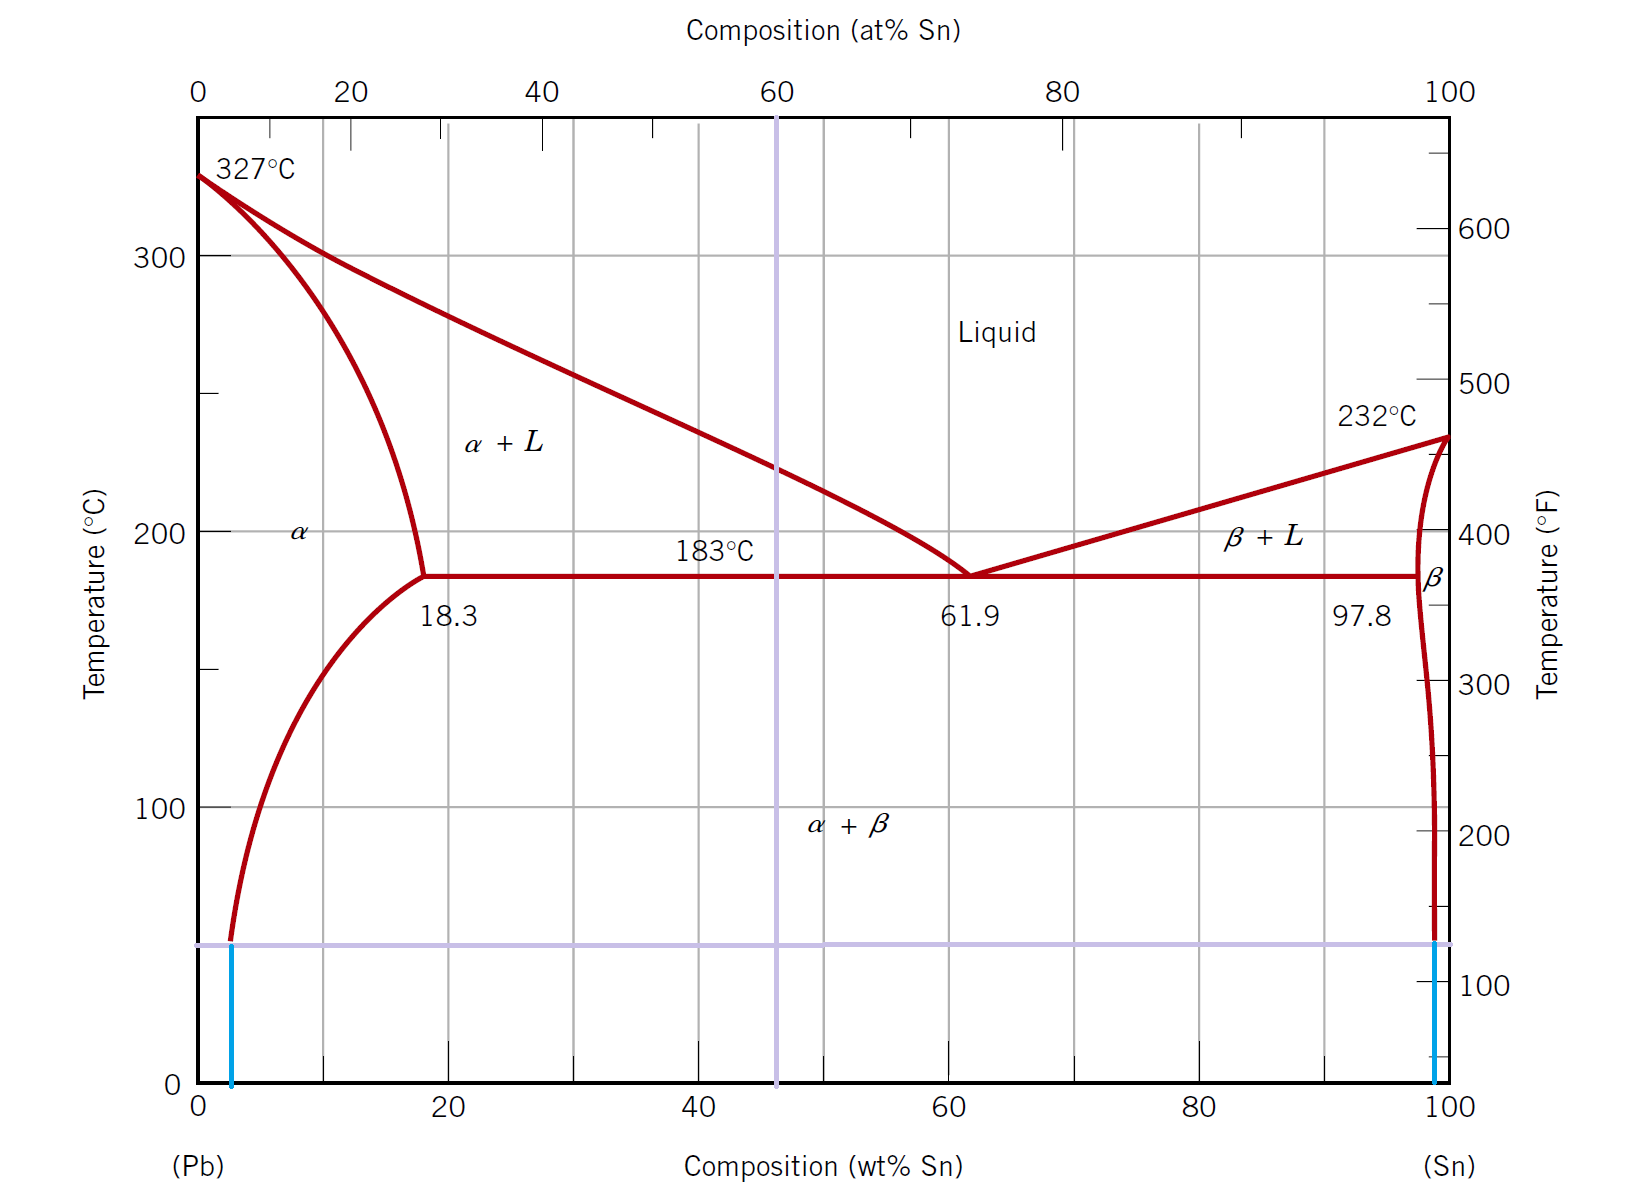
\includegraphics[width=1\textwidth]{graficas/diagrama.png}
%    \caption{Phase diagram for lead-tin \\
%    \textit{Source: Figure adapted from \citep{callister2010materials}}}
%    \label{fig:diagrama}
%\end{figure}

\begin{mdframed}
The volumen fraction of the primary phase is 0.68.
\end{mdframed}

\newpage
\subsection{}
A Pb–$25$ at$\%$ Sn alloy was slowly cooled from 380°C to 50°C. Ideally, Sn phase is expected to precipitate within Pb-phase grains, but in reality, a eutectic structure appeared. Assuming there were no experimental issues such as weighing errors, discuss the reason why this phenomenon occurred.

%\begin{mdframed}
\shnote{Aca creo que deberia de ir la discusion del punto eutectico, pero ahorita no me acuerdo por que es que se forma esa cosa :c}
%\end{mdframed}
\newpage
\section{}

\subsection{}
Pure water was quasi-statically cooled from room temperature to $-5^{\circ}$C under $1$ atm pressure. Calculate the critical nucleus radius under these conditions. Assume the nucleus is spherical, the latent heat is $6$ kJ/mol, the interfacial energy between ice and water is $30$ mJ/m$^2$, and the density of ice is $1$ g/cm$^3$.

The critical nucleus radius can be calculated using the following equation \citet{callister2010materials}: 
\begin{align}
  \label{eq:r01}
  r^*&=\dfrac{-2\gamma}{\Delta G_v},
\end{align}

where $\gamma$ is the surface free energy, and $\Delta G_v$ is the volume free energy change. Because $\Delta G_v$ is a function of temperature:
\begin{align}
  \label{eq:deltagv}
  \Delta G_v&= \dfrac{\Delta H_f\left(T_m-T\right)}{T_m}.
\end{align}

Substituting equation \ref{eq:deltagv} in \ref{eq:r01} gives: 
\begin{align}
  \label{eq:nucleus_radius}
  r^*&=\left(\dfrac{-2\gamma T_m}{\Delta H_f}\right)\left(\dfrac{1}{T_m - T}\right),
\end{align}
where $\gamma$ is the surface free energy, $\Delta H_f$ is the the latent heat of fusion, $T_m$ is the melting temperature and $T$ is the transformation temperature.

The critcal nucleus radius for water quasi-statically cooled from room temperature to $-5^{\circ}$ is:
\begin{align}
  \label{eq:radius}
  r^*&=\left(\dfrac{-2*0.03*273}{6000}\right)\left(\dfrac{1}{273-268}\right)=
\end{align}

\subsection{}
Explain how the critical nucleus radius changes if the pure water is
further cooled, including the reason.

To visualize the changes of the radius with further cooling water, 

(Aca creo que podria calcular el radio para mas temperaturas y talvez graficar eso y mostrar la tendencia y asi)
\clearpage
\section{Diffusion Distance}

The diffusion distance is given by $\sqrt{Dt}$, which is found in the equation that is used to describe the concentration after a time $t$ in a thin layer of the diffusing species is concentrated at $x=0$ of a semi-infinte sample \cite{diff}:
\begin{align}
  \label{eq:3}
  c(x,t)&=\dfrac{M}{\sqrt{\pi D t} \exp\left(-\dfrac{x^2}{4DT}\right)}.
\end{align}

Using the previous statement, the difussion distance was calculated using a time range from zero to (tengo que arreglar esta parte, porque creo que meti la pata con el calculo del tiempo :c). The plots for the diffusion distance as a function of time and the lilnealization of the diffusion distance are shown in the figure \ref{fig:length}.

\subsection{Self-diffusion}

The shoshfdos

\begin{figure}[h]
 \centering
 \captionsetup{justification=centering}
  \subfloat[]{
   \label{fig:d}
    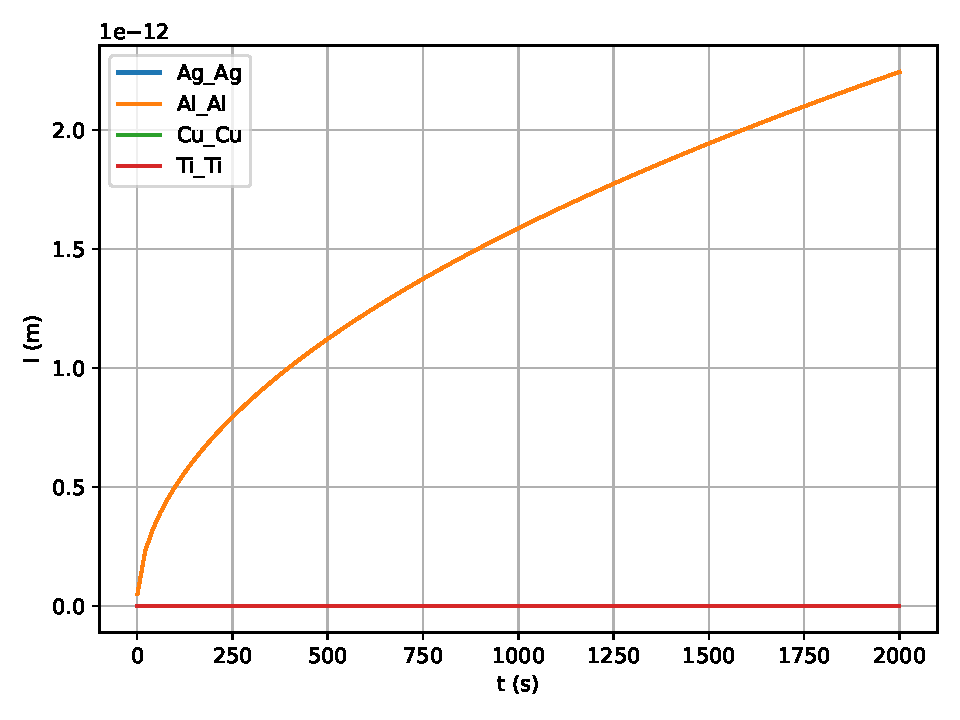
\includegraphics[width=0.5\textwidth]{graficas/l_self.pdf}}
  \subfloat[]{
   \label{fig:lnd}
    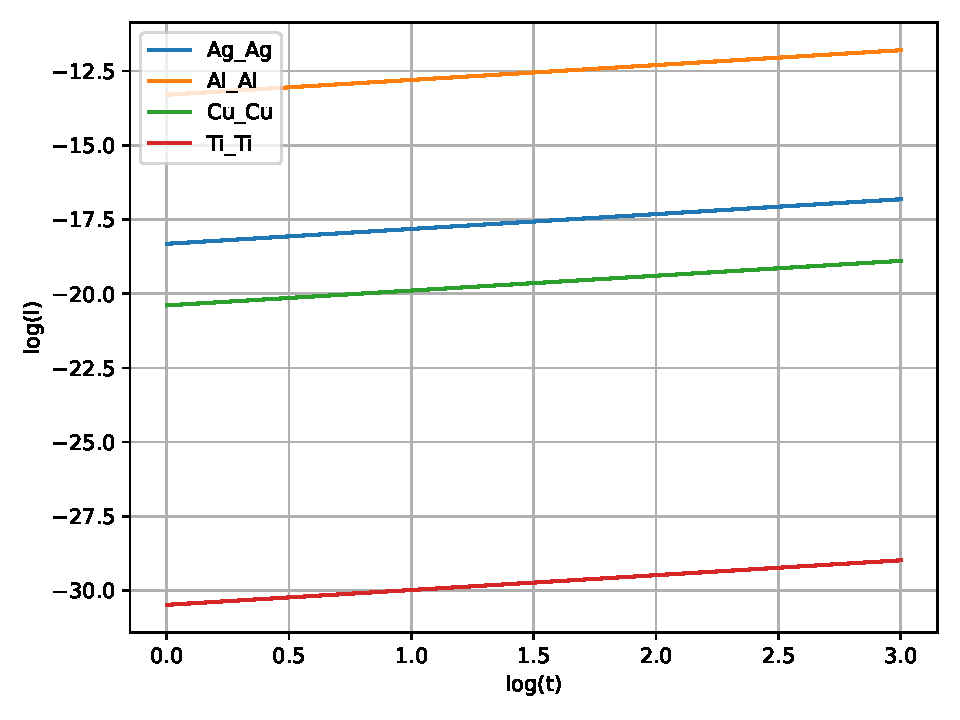
\includegraphics[width=0.5\textwidth]{graficas/log(l)_self.pdf}}
 \caption{a) Diffusion coefficient $D$ ($m^2/s)$ as a function of temperature $T$ (K) and b) logarithm of the diffusion coefficient $ln(D)$ as a function of the inverse of temperature $1/T$ ($K^{-1}$). \\
 \textit{Source: Data from \citep{kakusan}, visualization by the author (code available at \citep{mygit}).}}
 \label{fig:diffusion}
\end{figure}


\subsection{Solute diffusion}

The fsdfojsofdjsodfs

\begin{figure}[h]
 \centering
 \captionsetup{justification=centering}
  \subfloat[]{
   \label{fig:d}
    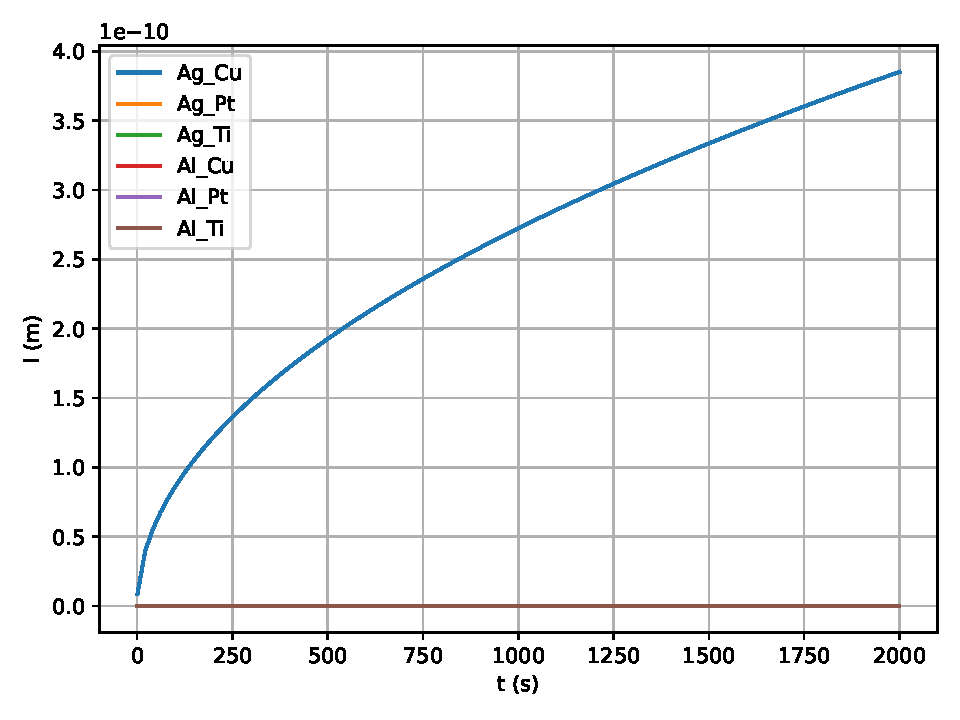
\includegraphics[width=0.5\textwidth]{graficas/l_other.pdf}}
  \subfloat[]{
   \label{fig:lnd}
    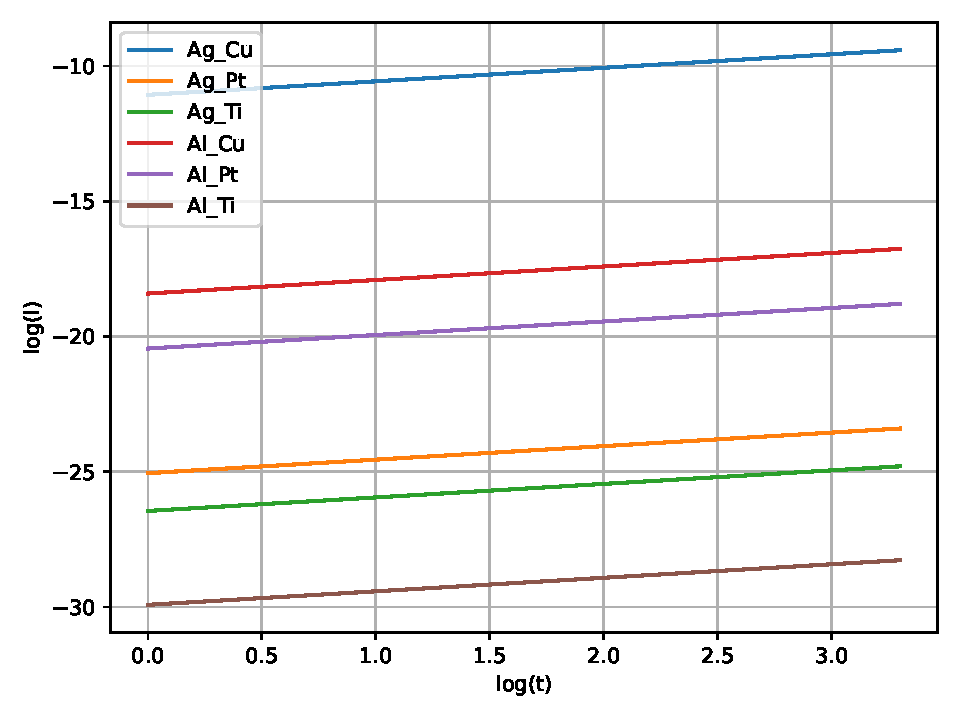
\includegraphics[width=0.5\textwidth]{graficas/log(l)_other.pdf}}
 \caption{a) Diffusion coefficient $D$ ($m^2/s)$ as a function of temperature $T$ (K) and b) logarithm of the diffusion coefficient $ln(D)$ as a function of the inverse of temperature $1/T$ ($K^{-1}$). \\
 \textit{Source: Data from \citep{kakusan}, visualization by the author (code available at \citep{mygit}).}}
 \label{fig:diffusion}
\end{figure}



%How far atoms have diffused in a given time.

%The rate of atomic motion in each material.

%Observations:
%Ag_Ag shows the highest diffusion length → silver atoms move the farthest in the same time → highest self-diffusivity.

%Ti_Ti shows the lowest diffusion length → titanium atoms diffuse more slowly.

%The curves are non-linear (parabolic), reflecting the square-root time dependence from the formula above.
\newpage
\section{Discussion}

(d) From questions (b) and (c), you will be able to see how the diffusion coefficients and diffusion distance depend on the types of metals and solute atoms. Discuss the origins of this dependence.
\bibliographystyle{abbrv}
\bibliography{references}


% --------------------------------------------------------------
%     You don't have to mess with anything below this line.
% -------------------------------------------------------------- 
\end{document}